\documentclass[10 pt]{article}
\usepackage[a4paper, total={7in, 9.5in}]{geometry}
\usepackage[spanish]{babel}
\usepackage{csquotes}
\usepackage{graphicx} 
\usepackage{caption}
\usepackage{hyperref}
\usepackage{graphicx}
\usepackage{float}
\usepackage{url}
\usepackage{color}
\usepackage{siunitx}
\usepackage{hhline}
\usepackage{multirow}
\usepackage{natbib}
\bibliographystyle{plainnat}
\usepackage{todonotes}




\begin{document}

\begin{titlepage}

\begin{center}
\vspace*{-0.5in}
\begin{figure}[htb]
\begin{center}

\includegraphics[scale=.3]{imagenes/uba2.jpg}
\end{center}
\end{figure}

\begin{large}
Maestría en Explotación de Datos y Descubrimiento del Conocimiento\\
\vspace*{0.15in}
Universidad de Buenos Aires \\

\vspace*{0.6in}
\end{large}

\begin{large}
Reporte sobre el trabajo de especialización\\
(ejercitación en Látex)\\

\end{large}
\vspace*{0.2in}
\vspace*{0.3in}

\begin{large}
Asignatura: Taller de tesis II \\
\end{large}

\vspace*{0.3in}
\rule{80mm}{0.1mm}\\
\vspace*{0.1in}
\begin{large}
Victoria Colombo

\vspace*{0.3in}

\vspace*{0.1in}octubre 2021
\end{large}
\end{center}

\end{titlepage}


\newpage

\section*{Resumen}

En este reporte doy cuenta de los avances de mi trabajo de especialización durante el segundo cuatrimestre de 2021. Dado el estado inicial de esta investigación, el presente reporte se limita a describir y problematizar brevemente los datos y a mostrar un análisis exploratorio parcial de ellos. El \textit{dataset} elegido se compone de llamados a la línea nacional 137 para denunciar casos de violencia sexual entre enero de 2016 y julio de 2021. Dada la particular naturaleza de los datos existen cuestiones sociales que lo atraviesan y que inevitablemente serán problematizadas a lo largo del análisis. Me refiero con esto a la violencia de género y su relación con la violencia sexual, y complementariamente a las dificultades para recopilar y luego acceder a datos de este tipo que, en última instancia, impiden la correcta implementación de mecanismos de asistencia y prevención la violencia de género. Teniendo en cuenta lo dicho, me propongo en este trabajo, sin dejar de centrarme en técnicas de limpieza, procesamiento y representación de datos, fundamentar mi análisis en bibliografía sobre violencia de género y violencia sexual ya existente e intentar aportar al estudio de estos temas desde la ciencia de datos.



\section*{Introducción}\label{intro}

En general los datos sobre delitos sexuales son difíciles de recabar, no necesariamente por su naturaleza sino por el contexto social que los rodea. A las víctimas a menudo no se les ofrece empatía, contención ni un lugar seguro para relatar y denunciar lo sucedido, muchas veces son re victimizadas por el sistema judicial y/o por la sociedad misma y algunas veces, como se muestra en el documental Línea 137 \citep{vasallo2020linea137}, no reconocen algunas situaciones de violencia sexual. Esto puede tener que ver en parte con el ocultamiento de ese tipo de violencia cuando ocurre, la naturalización si la violencia se da al interior de una pareja y la falta de educación sexual no solo o no necesariamente de la víctima sino de su entorno social en general \citep{contreras2016violencia}. Al mismo tiempo, recopilar y analizar estos datos para tener información estadística confiable sobre la problemática es importante para poder pensar e implementar soluciones efectivas.

El programa Las Víctimas contra las Violencias depende del Ministerio de Justicia y Derechos Humanos de la Nación y fue creado en el año 2006 con el objetivo de brindar atención e intervención institucional a víctimas de abusos y violencia familiar o sexual\footnote{Dentro de la categoría de violencia familiar se incluyen varios tipos de violencia, entre ellos, la sexual}. Para denunciar y solicitar asistencia las víctimas cuentan, desde 2016, con la línea nacional de emergencia 137 que funciona las 24 horas del día, todo el año, y cuenta en al menos cinco ciudades del país con equipos especializados para llevar a cabo el acompañamiento y las intervenciones necesarias. Los registros de esas llamadas e intervenciones se encuentran digitalizados al menos desde 2017 y están disponibles en el \href{http://datos.jus.gob.ar/}{Portal de Datos Abiertos de la Justicia Argentina}. Allí se recopilan bajo la clasificación de llamados e intervenciones domiciliarias por situaciones de violencia familiar y llamados e intervenciones domiciliarias por situaciones de violencia sexual. 

Para este trabajo he tomado en principio los llamados de denuncias por violencia sexual desde enero de 2017 hasta julio de 2021. El \textit{dataset} se compone en total de 19143 observaciones y 54 variables, en su mayoría categóricas, que aportan información sobre la víctima, la persona denunciante, el contexto del hecho y el tipo de violencia sufrida. En la tabla \ref{tablavar} se detallan las variables y su tipo.




\begin{table}[ht!]
\centering
\caption{Resumen de las variables.}
\label{tablavar}
\begin{tabular}{|l|l|l|l|} 
\hline
Descriptor & Tipo variable & Variables & Observaciones         
\\ 
\hline
\multirow{2}{*}{Víctima} & Cuantitativa & victima\_edad &  
\\ 
\cline{2-4}
 & Cualitativa & \begin{tabular}[c]{@{}l@{}}victima\_genero, victima\_nacionalidad, \\ victima\_discapacidad,\\ victima\_vinculo\_agresor,\\victima\_convive\_agresor,\\ victima\_a\_resguardo\end{tabular} & \begin{tabular}[c]{@{}l@{}}victima\_genero toma los valores: \\masculino, femenino, trans, \\ NS/NC.\end{tabular}           
 \\ 
\hline
\multirow{2}{*}{Llamante} & Cuantitativa         & {llamante\_edad}&               \\ 
\cline{2-4}
 & Cualitativa& llamante\_genero, llamante\_vinculo & \begin{tabular}[c]{@{}l@{}}llamante\_genero toma los valores: \\masculino, femenino, trans, \\ NS/NC.\\llamante\_vinculo\_ refiere a vínculo \\con la víctima.\end{tabular}                \\ 
\hline
\multirow{2}{*}{Llamado}& Cuantitativa & llamado\_fecha\_hora&                                             \\ 
\cline{2-4} & Cualitativa & \begin{tabular}[c]{@{}l@{}} caso\_id, llamado\_provincia, \\ llamado\_provincia\_id, \\ caso\_judicializado, hecho\_lugar\end{tabular} & \begin{tabular}[c]{@{}l@{}} llamado\_provincia\_id refiere al id \\numérico para las provincias \\según codificación INDEC.\end{tabular}                                \\ 
\hline
Violencia sexual                 & Cualitativa  &  \begin{tabular}[c]{@{}l@{}} vs\_violacion\_via\_vaginal, \\ vs\_violacion\_via\_anal, \\ vs\_violacion\_via\_oral, \\ vs\_tentativa\_violacion, \\ vs\_tocamiento\_sexual, \\ vs\_intento\_tocamiento, \\ vs\_intento\_violacion\_tercera\_persona, \\ vs\_grooming, vs\_exhibicionismo, \\ vs\_amenazas\_verbales\_contenido\_sexual, \\ vs\_explotacion\_sexual, \\ vs\_explotacion\_sexual\_comercial, \\ vs\_explotacion\_sexual\_viajes\_turismo,\\ vs\_sospecha\_trata\_personas- \\ \_fines\_sexuales, \\ vs\_existencia\_facilitador-\\
\_corrupcion\_nnya, \\ vs\_obligacion\_sacarse\_fotos\_pornograficas, \\ vs\_eyaculacion\_partes\_cuerpo, \\ vs\_acoso\_sexual, \\ vs\_iniciacion\_sexual\_forzada\_inducida, \\ vs\_otra\_forma\_violencia\_sexual, \\ vs\_no\_sabe\_no\_contesta \end{tabular} &

\begin{tabular}[b]{@{}l@{}} vs\_existencia\_facilitador-\\
\_corrupcion\_nnya \\ refiere a la existencia de un \\ facilitador de la corrupción de \\ niños, niñas y adolescentes.\\\\ vs\_no\_sabe\_no\_contesta refiere \\ violencia sexual que se desconoce \\ o que no hace referencia a los otros \\ campos mencionados.\end{tabular}                                                  \\ 
\hline
Otras violencias & Cualitativa & \begin{tabular}[c]{@{}l@{}} ofv\_sentimiento\_amenaza, \\ ofv\_amenazas\_explicitas, \\ ofv\_violencia\_fisica, ofv\_intento\_ahorcar, \\ ofv\_intento\_quemar,  ofv\_intento\_ahogar, \\ ofv\_amenaza\_muerte, \\ ofv\_uso\_sustancias\_psicoactivas, \\ ofv\_intento\_privacion\_libertad, \\ ofv\_privacion\_libertad, \\ ofv\_uso\_arma\_blanca, \\ ofv\_uso\_arma\_fuego, \\ ofv\_enganio\_seduccion, ofv\_intento\_matar, \\ ofv\_uso\_animal\_victimizar, \\ ofv\_grooming, ofv\_otra\_forma\_violencia, \\ ofv\_no\_sabe\_no\_contesta\end{tabular} &  \\ 
\hline
\end{tabular}
\end{table}




\section{Metodología}\label{met}

Los datos de los llamados desde 2017 hasta julio de 2021 fueron descargados del portal mencionado en la sección anterior en cinco archivos de formato csv separados, uno por año. La unificación de esos archivos en un solo \textit{dataset} implicó realizar algunas modificaciones para sortear problemas de correspondencias entre años. La variable \textit{caso\_id} solo existe desde el primer trimestre de 2020, los casos anteriores a esa fecha no contaban con ella, por lo tanto tomé la decisión de eliminarla también para 2020 y 2021. La variable \textit{llamado\_provincia\_id} llevaba otro nombre hasta el año 2019: \textit{llamado\_provincia\_indec\_id} y fue entonces modificada en 2017, 2018 y 2019 para llevar el nombre actual. 
\newline
Los \textit{types} de las variables cualitativas fueron cambiados a \textit{categorical}\footnote{El análisis exploratorio y el resto del trabajo con datos fue y será realizado en Python} \todo{esto va en metodología}. Además, los valores que tomaban al menos 9 de esas variables categóricas debieron ser normalizados por errores varios en la carga o valores cargados con sinónimos. Por ejemplo, muchos NS/NC fueron cargados en minúscula y en mayúscula en la misma columna y debieron ser normalizados a mayúscula; además, por ejemplo en la variable \textit{victima\_vinculo\_agresor} se repetían algunos valores cargados con distinta ortografía como "Ex pareja de la víctima" y "Ex-pareja de la víctima" y "Expareja de la víctima" que debieron ser normalizados.
Los \textit{types} de las variables cuantitativas de edad fueron pasados a \textit{integer}. Los valores numéricos de \textit{victima\_edad} y \textit{llamante\_edad} tenían errores de carga evidentes ya que aparecían valores numéricos demasiado altos para ser edades como: 125, 221, 324. Las filas con esos valores no fueron eliminadas por el momento porque considero que el resto de los datos de la fila no están errados y es posible que los necesite más adelante. En cambio, los datos fueron marcados para no ser utilizados en análisis que incluyan las variables de edad.
A modo de análisis exploratorio, realicé histogramas univariados para ver la frecuencia de las categorías de las variables: \textit{victima\_genero}, \textit{victima\_discapacidad}, \textit{victima\_convive\_agresor}, \textit{victima\_vinculo\_agresor}, \textit{llamante\_edad}, \textit{llamante\_genero}, \textit{llamante\_vinculo} y \textit{hecho\_lugar}. Además, realicé un agrupamiento de las categorías de vínculos entre agresor y víctima para poder distinguir entre parejas, familiares y no familiares (conocidos). Algunos de estos histogramas se comentan en la sección siguiente. 

Me propongo como continuación de este análisis explorar la fecha y hora de los llamados, las edades de las víctimas y llamantes, las formas de violencia más comunes, y construir una variable de género del agresor utilizando la variable que estipula el vínculo entre la víctima y el agresor, ya que en algunas de sus categorías el género se encuentra expresado inequívocamente (por ejemplo en las categorías padre, madre, hermano). Además, me interesa sumar análisis multivariados para ver la interacción entre algunas de las variables. Por último, tengo la intención de investigar asociaciones entre variables como edad de la víctima y vínculo con el agresor.

\section{Resultados}\label{res}

Al mirar la variable de género de la víctima se evidencia que aproximadamente el 80\% de ellas son mujeres (ver figura \ref{generovict}), dato que no resulta sorprendente para la problemática de violencia sexual. Sin embargo, es importante tener en cuenta que si los delitos de violencia sexual son poco denunciados, lo son menos cuando las víctimas son varones y mucho menos cuando las víctimas son mujeres u hombres transgénero.\footnote{En este punto me gustaría hacer hincapié en un problema del diseño y la metodología de la recopilación de datos para este \textit{dataset}; la categoría transgénero no especifica si se trata de un hombre o una mujer transgénero. } 


\begin{figure}[H]
\begin{center}
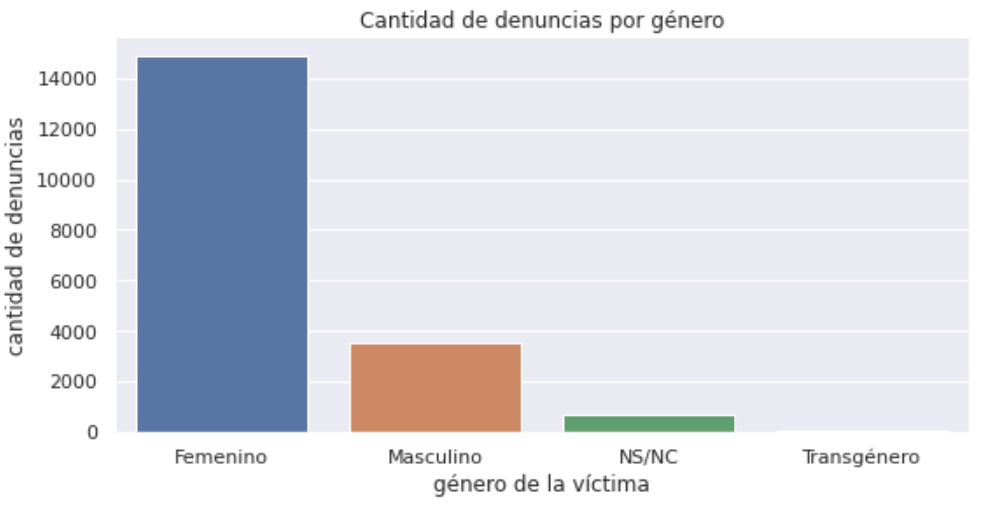
\includegraphics[scale=.29]{imagenes/cantidad_denuncias_genero.png}
\vspace{1.5em}
\caption{Distribución de género en las víctimas.}
\vspace{1.5em}
\label{generovict}
\end{center}
\end{figure}

Al explorar la variable de vínculo con el agresor en la figura \ref{vinculos} se ve una distribución bastante dispersa entre distintas categorías que implican miembros de la familia, parejas o ex parejas, conocidos no familiares, una gran cantidad de casos en que el agresor es desconocido, y también una gran cantidad con la respuesta NS/NC. Con la intención de hacer foco en la distinción entre vínculos familiares, vínculos no familiares, vínculos sexo-afectivos y los casos NS/NC, en la figura \ref{vinculosagrupados} agrupé las categorías de la siguiente manera: 

\begin{itemize}
    \item Familiar: abuela, abuelo, hermana, hermano, madrastra, madre, padrastro, padre, tío, otro pariente
    \item No familiar: desconocido, conocido no familiar
    \item Pareja/Ex: pareja de la víctima, ex pareja de la víctima
\end{itemize}

Puede verse ahora con este nuevo agrupamiento la prevalencia de vínculos familiares con los agresores, una estadística conocida y reportada en varios estudios\citep{argentina2016analisis}, \citep{contreras2016violencia}. Cabe además preguntarse por la cantidad de NS/NC y la cantidad de Desconocido que si bien en la figura \ref{vinculosagrupados} quedó absorbida en la categoría No familiar, en la figura \ref{vinculos} resultaba una categoría muy prominente. Nuevamente, el tipo de datos con los que estoy trabajando y la forma en que son recopilados dificulta las conclusiones sobre estos resultados; una posible hipótesis es que las verdaderas identidades de los agresores sean ocultadas en muchos casos por quien denuncia para proteger a familiares o incluso a las propias víctimas.\footnote{Un ejemplo de esta situación se puede ver en el documental Línea 137\citep{vasallo2020linea137}}

\begin{figure}
\begin{center}
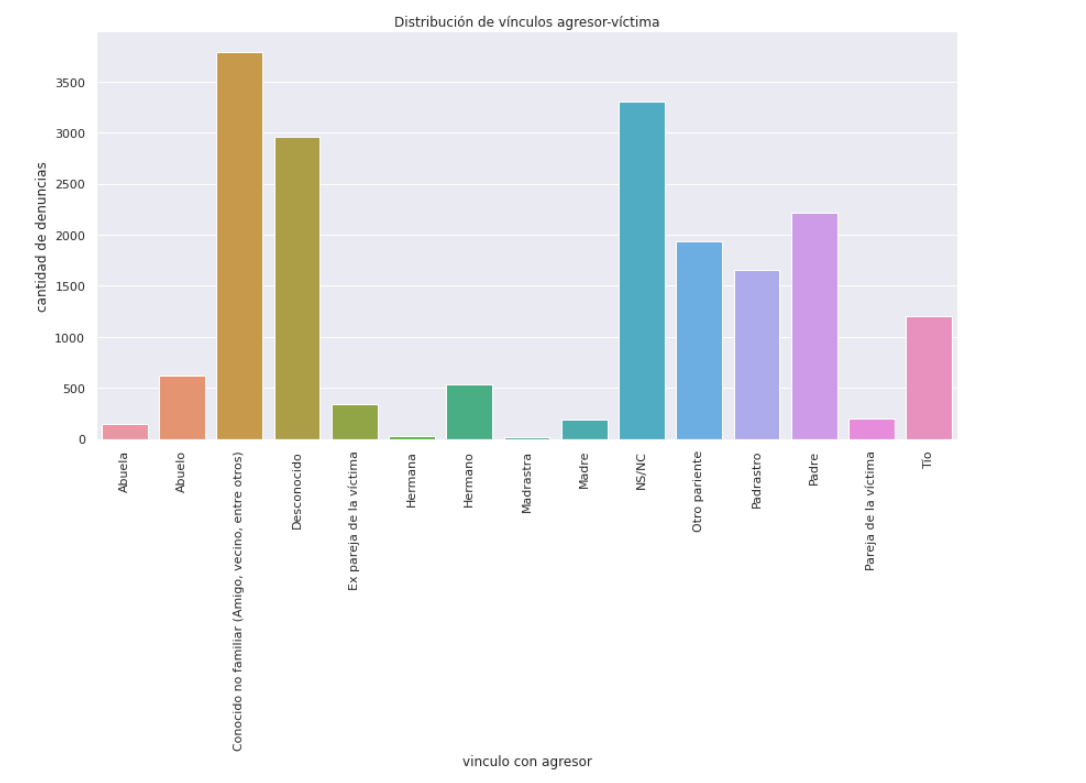
\includegraphics[scale=.29]{imagenes/distribucion_vinculos_agresor_vctima.png}
\vspace{-1em}
\caption{Distribución de vínculos entre agresores y víctimas.}
\vspace{-1.5em}
\label{vinculos}
\end{center}
\end{figure}

\begin{figure}[H]
\begin{center}
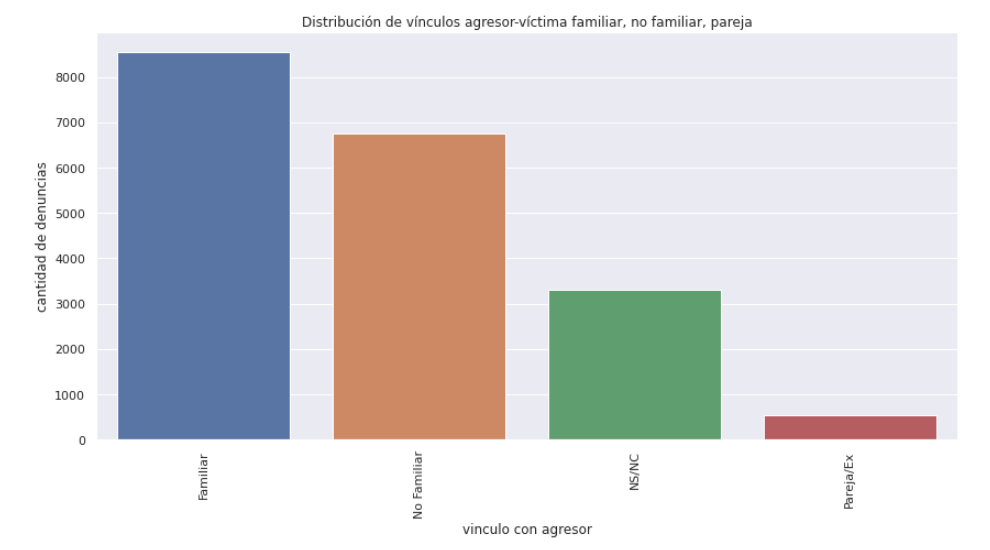
\includegraphics[scale=.29]{imagenes/vinculos_agresor_victima_agrupado.png}
\vspace{1.5em}
\caption{Distribución de vínculos entre agresores y víctimas agrupados.}
\vspace{1.5em}
\label{vinculosagrupados}
\end{center}
\end{figure}

\newpage

\bibliography{bibtex_reporte.bib}

\end{document}